\documentclass[conference]{IEEEtran}
\usepackage{graphicx}
\usepackage{url}
\usepackage{pbox}
\usepackage{xcolor}
%\usepackage[colorlinks]{hyperref}
%\hypersetup{linkcolor=blue, citecolor=blue, urlcolor=blue}

\DeclareGraphicsExtensions{.pdf,.png,.jpg}
\graphicspath{{./ImportedFigures/}}

\ifCLASSINFOpdf
\else
\fi
\hyphenation{op-tical net-works semi-conduc-tor}

\newif\ifdraft
\drafttrue
\ifdraft
\usepackage{xcolor}
\usepackage{array}
\usepackage{makecell}
\renewcommand\cellalign{cl}
\definecolor{ocolor}{rgb}{1,0,0.4}
\newcommand{\aanote}[1]{ {\textcolor{red} { ***amy: #1 }}}
\newcommand{\alnote}[1]{ {\textcolor{blue} { ***andre: #1 }}}
\newcommand{\ednote}[1]{ {\textcolor{brown} { ***eddie: #1 }}}
\newcommand{\kknote}[1]{ {\textcolor{green} { ***ken: #1 }}}
\newcommand{\dungnote}[1]{ {\textcolor{orange} { ***dung: #1 }}}
\else
\newcommand{\aanote}[1]{}
\newcommand{\alnote}[1]{}
\newcommand{\ednote}[1]{}
\newcommand{\kknote}[1]{}
\newcommand{\dungnote}[1]{}
\fi

\begin{document}

\title{Edge Processing of Deep Learning Computer Vision Applications in  Automotive Manufacturing}
% * <dungx.ngt@gmail.com> 2017-10-02T03:34:15.504Z:
%
% ^.


\maketitle

% These two lines add back the page numbers; we may nhttps://v2.overleaf.com/9174271949jhbybhjxjrsbeed to remove
% before submitting
\thispagestyle{plain}
\pagestyle{plain}



\begin{abstract}
In this paper, we investigate the trade-off between resource/cost consumption with running time and accuracy of different object detector models based on deep neural networks.
Execution is in an automotive manufacturing environment that places deadlines on the completion of the object detection application.  
\end{abstract}


\IEEEpeerreviewmaketitle

\nocite{*}

%%%%%%%%%%%%%%%%%%%%%%%%%%%%%%%%%%%%%%%%%%%%%%%%%%%%%%
\section{Introduction and Motivating Application}
%%%%%%%%%%%%%%%%%%%%%%%%%%%%%%%%%%%%%%%%%%%%%%%%%%%%%%

Deep learning system have become pervasive in the automotive domain. For example, an increasing number of visual inspection tasks in automotive manufacturing is conducted using camera-based systems and different kinds of classifier, detection and segmentation networks. A challenge is the data-intensiveness and computational complexity of these algorithms. One challenge is the deployment of this tools in the business process. As these algorithms are typically run on the edge device to ensure real-time feedback and the ability to react on the results in the business process. At the same time the usage of cloud is important to (i) utilize more complex deep learning models for higher accuracies and (ii) to combine data with other data, such as process and data from further sensors.


We aim to compare different families of object detectors in different devices: from state-of-the-art multiple GPUs workstations to resource-limited devices such as mini computers (Raspberry Pi, NIVDIA ...) and mobile devices (iPhone) or deep learning-specialized devices (Amazon DeepLens).

% Minicomputer -> embedded
% Devices 

\alnote{Motivate streaming}

The difficulties of this project come from the differences of deep learning framework environments on different devices with different levels of optimization and efficiency, the wide varieties of object detectors, in both meta-architectures and feature extractors, and the constraints of the execution environment that imposes hard deadlines on the completion of the object detection methods.

For our applications, we only consider the test-time performance, which concerns about inference time, deployment time, memory footprint and hardware utilization in test-time only.

We illustrate a big picture of deep network object detectors for many different devices and purposes. Very light-weight devices such as Raspberry Pi require a small network and efficient run time environment to produce minimal memory footprint. Other devices requires real-time processing time to provide smooth user experience, particularly on smartphones. Different applications and devices have their own unique requirements and characteristics. 

%%%%%%%%%%%%%%%%%%%%%%%%%%%%%%%%%%%%%%%%%%%%%%%%%%%%%%
\section{Architecture Backgrounds}
%%%%%%%%%%%%%%%%%%%%%%%%%%%%%%%%%%%%%%%%%%%%%%%%%%%%%%

Traditionally, Computer Vision applications used to be implemented by training machine learning models to low-level features such as SIFT. It requires complex feature engineering tasks to produce effective feature sets for different kinds of application. Nowadays, deep learning techniques are widely adopted due to their simplicity in image processing: They can be applied directly to raw images without complex feature extraction algorithms. Many common tasks such as image classification and object detection can be solved effectively using out-of-the-box deep learning architectures.

Among deep learning applications, Computer vision applications requires relatively small amount of pre-processing tasks in comparison with other fields such as natural language processing or speech recognition. The only required pre-processing is to make sure all pixels are in the same scale. A typical pre-processing task is contrast normalization, which is proportional with L-2 normalization of "each" pic: subtracting the mean and divided by standard deviation. It can be done in global (the whole picture) or local. 

Contrast normalization (~L-2 normalization) makes all data points have the same (or similar) vector size (same norm). It makes learning more feasible because neural units react better with directions in space with different sets of coefs and worse with distance (bias). It is also beneficial to augment the dataset with different transformations of images (like rotating, cropping, adding noise) to have better generalization.

Computer vision exploits convolutional networks to produce state-of-the-art results in many applications, such as image classification or object detection.

Convolutional networks are neural networks that use a convolutional function between input and a kernel. The kernel works like a mask, iterates all over the spatial space of an input layer. Convolutional networks leverages 3 important ideas: sparse connections, parameter sharing and equivariant representations.

Usually, after each convolution layer, there is an activate layer (i.e reclu) and a pooling layer, which aggregate results from several nearby elements. The pooling layer helps increase the invariant of output to input.

Pooling is a special step in convolutional layer. It groups several elements and applies a function to them. Spatial function works with nearby elements in spatial space, while multi-channel pool groups elements from independently learned parameters (from different kernel).

Convolutional networks create very huge capacity networks, but constraints the weights to be mostly zeros (because kernels are relatively small in sizes) and equal to other (many parts of data input shares same kernel weights).

\begin{figure*}[htpb]
	  \centering
	  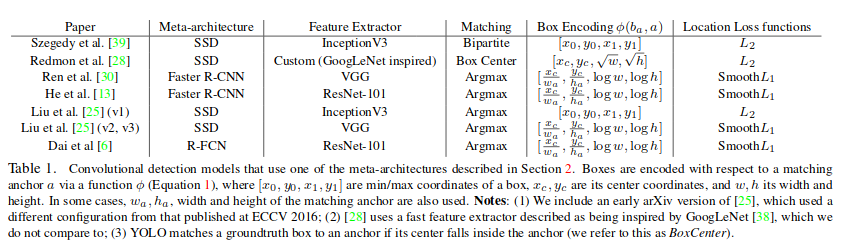
\includegraphics[width=\textwidth]{original_models}
	  \caption{\textbf{Original models with their attributes.}}
	  \label{fig:original_models}
\end{figure*}

Object detection is a popular task that convolutional networks can solve effectively. Many different architectures are proposed in recent years, which have different characteristics. Some models are designed to achieve state-of-the-art performance in accuracy. Several models aim to get reasonable accuracy within limited time and computational resources. There are efforts to build deep learning models for special hardware systems (FPGA) or resource-limited devices such as smartphones. There are multiple degrees of freedom in object detection architectures which affect their accuracy, running time and required resources:

\begin{itemize}
    \item Meta-Architecture: SSD, DeepMultiBox, R-FCN, Faster R-CNN, YOLO, ... which is categorized into single stage and 2-stage classes.
    \item Feature Extractor: VGG (multiple versions), Resnet (m), Inception (m), Inception Resnet, MobileNet. At least 6 are reported in~\cite{huang2017speed}. Feature Extractors are usually image classification networks which are pre-trained on common dataset such as ImageNet-CLS (Image Classification dataset) first, and then are used to initialize the complete networks. 
    \item Feature Layers: Select which layer(s) of the feature extractor to be used in Meta-Architecture. Several papers select the top (deepest) convolutional layer, but other papers encourage to aggregate multiple layers, even fully-connected layers.
    \item Box Proposals: Different original paper reports different number of proposals, as well as how to select proposals (10 .. 300 for an image of ~300x300 pixels)
    \item Trained Image size: 300 .. 600: R-FCN and Faster R-CNN are fixed at shorter edge. SSD is fixed at both edges.
    \item Stride (in feature extractor): reports show that stride is an important factor in the trade-off between performance (in mAP) and running time.
    \item Data Augmentation: Methods to transform images (rotation, cropping, etc) to make the models more robust.
\end{itemize}

Original papers usually just report 1 single combination of these options, with several variants such as different image resolutions, the numbers and positions of the candidate boxes, the layers from which features are extracted and the number of layers.

\dungnote{A strong argument against using original models but not combinations is the original models are optimized to get highest accuracy but not taking into account other trade-off such as memory or inference time. Several original models use different complex data augmentation methods. Another issue is original papers report results on different combinations of training sets (2007/2012 PASCAL VOC eval, 2007+2012 PASCAL VOC eval + test, etc}

\dungnote{A good thing is the paper at~\cite{huang2017speed} already produced a pipeline to re-train all the setup combinations. Therefore we only need to add/implement parts of new combinations. Source code can be found on Github. Training/Evaluation can be done only once in powerful workstations. We only need to record running time and resource utilization at edge devices.}

\dungnote{Pytorch doesn't have officially hosted trained models for object detections. They only have several image classification models in their official repository.}

\subsection{Meta-Architectures}

% \alnote{good practical overview: \url{https://github.com/datadynamo/aiconf_ny_2018_pytorch_cv_tutorial/blob/master/AIConf_April2018_PyTorch_Computer_Vision_Part2.pdf}}

% \alnote{Yolo v3?}
Meta-architectures in object detection models can be categorized into 2 different classes: single stage and 2-stage. In 2-stage models, images are passed through a first parts to produce box proposals (which are rectangle parts of the input images) and then the proposals are feed into the second stage to predict objects and re-calulate the bounding boxes. In single stage models, input images are passed through the networks once to produce predicted objects and their bounding boxes.

In general, single stage meta-architectures such as SSD and YOLOv2 are used for fast, low-latency jobs while 2-stage meta-architectures as Faster R-CNN and R-FCN are often used for better accuracy.

\subsubsection{DeepMultiBox}
DeepMultiBox is a box-generating model that becomes a basis for many other object detection architectures. Rather than a fully object detection model, it only predicts class-agnostic boxes with confident scores.

DeepMultiBox treats the class-agnostic bounding box as a regression problem of coordinates of boxes and their confident scores. The network predicts K boxes, with K is normally 100 or 200. Each box is described by 5 nodes in the last layer of the network, which are upper-left and bottom-right coordinates and a confident score in range $\{0, 1\}$.

To be faster and better in training, the ground truth boxes are clustered into K priors and the network will use the K priors as initilizations. Then, in the matching steps, rather than using the matches between predictions and ground truth boxes, the network uses the matches between these priors and ground truth ones. This process is called prior matching and is exploited by many other researches.

The original model uses the same neural architecture with AlexNet, only differs at the very top layer of the network. Loss function is calculated as weighted sum of localization errors and confident erros over all K prediction.


\subsubsection{YOLO and its variants}
YOLO also uses single neural network without proposal generation process, combined with a customized feature extractor derived from GoogLeNet to predict classes and shapes of objects.


\subsubsection{SSD}
SSD is one of the fastest meta-architectures, along with variants of Yolo. SSD is more flexible~\alnote{what does flexible mean?} ~\dungnote{in Yolo, at least to version 2, you can not choose where you get the features, they are fixed in the network. In SSD you can choose whatever layers you want. By the way, the word ``flexible'' is used by the authors of SSD so I just think it's okay to reuse it}than YOLO because it uses prior boxes at different aspect ratio at different scale of feature map.~\cite{liu2016ssd} Because of this attribute, SSD can detect objects at different scales in images.

The original models are trained on PASCAL VOC (2007 and 2012 versions) and 2014 ILRSVRC datasets. The image's resolutions used in the original paper are $229 \times 229$ and $443 \times 443$.

SSD is short for Single Shot Detector, which means that the information flows through only 1 single neural network architecture in the model. It is contrast with other meta-achitectures such as R-CNN based models and R-FCN models, in which they contain at least a second convolutional structure to refine the results from a box proposal generator. Because of this characteristic, SSD is usually faster than R-CNN based models and R-FCN models in several orders of magnitude and consume less resource to run~\cite{huang2017speed}.

SSD does not have box proposal steps but calculate the bounding boxes and object's classes at the same time in a single propagation. The prior boxes (or anchors) are fixed at multiple scales for all images and the network will try to correct the priors to find the most prominent box for each object.

From the optimization viewpoint, SSD calculate a single loss function for both bounding box localization and object classification errors using a weighted sum of 2 loss functions. 

Because of using prior boxes at different scales but not calculate the box proposals, SSD does not have good performance on small objects~\cite{liu2016ssd}.


\subsubsection{R-CNN }
R-CNN is a two-stage model to deal with object detection task: to generate bounded boxes and classify the object inside these boxes. The model is composed of three modules: Region Proposal, Feature Extraction and Region Classifications. Region Proposal module can be chosen from many methods already existed in literature, in which R-CNN chooses "selective search" to produce proposals. At inference time, the model produces 2000 proposals for each image. Feature Extraction transforms each region to a fix-sized feature vector by using the output of a hidden layer of a CNN model. Region Classification trains an SVM classifier, using fix-sized feature vectors produced by Feature Extraction.

Feature Extraction training is composed of two phases. The 1st phase is a supervised pre-training on an image classification task using a big dataset (where data are much more available). The 2nd phase replaces the output layer (because the incompatibility of the pre-training dataset and object detection dataset) then initializes the connection of last hidden layer with the new output layer and trains with box-bounded regions and their labels. A region's label is assigned to the ground-truth box's label for which they have more than 0.5 IoU overlap.

In the Region Classification, positive examples are ground-truth regions while negative examples are regions with less than 0.3 IoU overlap with the ground-truth ones.

R-CNN is originally pre-trained on PASCAL VOC 2007 and fine-tuned on PASCAL VOC 2012 datasets. 

\subsubsection{SPPnet}
SPPNet is an improved version of R-CNN to exploit the features produced by R-CNN convolutional network. This meta-architecture is faster than R-CNN but is out performed by Fast R-CNN and Faster R-CNN.

SPPnet enhances R-CNN by using a fixed-length feature maps, which are independent from the scale or resolution of images. In the last layers of feature networks, SPPNet applies spatial pyramid pooling layers to different regions of an image to create fixed-length feature maps.

The spatial pyramid pooling layers are placed in between convolutional layers and fully connected layers since convolutional layers can work with an abitrary size of input vectors, while the fully connected layers only work with fixed-length input vectors.

SPPnet has comparable accuracy with R-CNN but is much faster in term of inference time. Though being out-performed by other meta-architectures, SPPNet defines a new method to exploit feature vectors produced by convolutional networks. Fixed-length multi-layer feature vectors can capture highly sophisticated information from different scales and also works well with images of different resolutions.

\subsubsection{Fast R-CNN}
Fast R-CNN improves R-CNN and SPP Net by eliminating multi-stage learning. Fast R-CNN uses only one loss function for multi tasks (box creation, object detection). This architecture does not require an additional classifier such as SVM in R-CNN to classify boxes into categories. The classification task is embedded directly into the neural network structure of the model.

Fast R-CNN is an improvement architecture based on R-CNN and SPP Net. It uses the fixed-length feature vector from SPP Net to create more efficient features in feature extraction phase. Different from R-CNN, where each box proposal is passed through the network separately, Fast R-CNN passes the whole image through its convolutional network structure (VGG16) once and creates multiple ROI (Region of Interest) layers from multiple box proposals. Each ROI layer is associated with one proposal. The feature vectors extracted from ROI layers are passed through another neural network structure to calculate a single target value (of the loss function) for each box proposal.

Fast R-CNN also combines two tasks of object detection (object classification and box regression) into a single loss function. The unified loss function in Fast R-CNN is a weighted sum of a loss function of object classification error and another loss function of box regression error.

Another improvement of Fast R-CNN over R-CNN is using a softmax classifier rather than an SVM model in the final stage of classification. The softmax layers not only improves the accuracy of the model by a small margin but also combines two separated stages of the detector (a conv net and an svm model) in R-CNN into a single neural network structure. It makes the learning phase faster and more efficient, as well as a more straightforward prediction phase. 

Fast R-CNN still uses an external box proposals creation like R-CNN, which depends on an existed algorithm to create candidates for boxes. 

\subsubsection{Faster R-CNN}
Faster R-CNN, which yields high accuracy object detection results, is a model that derived from R-CNN~\cite{girshick2015fast}. Faster R-CNN is currently state-of-the-art meta-architecture in term of accuracy in object detection. Faster R-CNN eliminates the major drawback of Fast R-CNN, which is the dependency of Fast R-CNN on an external box proposals creator. By embedding the box proposal process into the neural network structure, Faster R-CNN increases both efficiency and accuracy of the previous models based on R-CNN.

Using a set of pre-defined anchor boxes as references, Faster R-CNN uses a part of the neural network structure to calculate the candidate box bounds and calls it Regional Proposal Network. This RPN shares components with the object detection network (Fast R-CNN) to utilizes calculated features from images. RPN and object detection network are trained separatedly. In inference time, box proposals are produced by RPN first, and then are passed through object detection network latter to form a 2-stage end-to-end object detector. Faster R-CNN is about an order of magnitude faster than Fast R-CNN while achieve better results on VOC dataset.

In training time, Faster R-CNN switches between region proposal optimization and object detection optimization. Because both tasks share a portion of the convolutional network, training time converges quickly. In inference time, the image is passed through the shared parts of the network first to produce (1) proposals that may contain objects and (2) feature maps used to predict objects and regress their bounding boxes. After getting results from proposal network, candidates go through another neural network structure to calculate prediction for objects and bounding boxes. The process above means Faster R-CNN is a two-stage detector, which requires 2 phases of computation and 2 seperated neural network sub-structures. 

Compared to Fast R-CNN, Faster R-CNN combines box proposal and object detection into a unified neural network structure, though they are still consisted of 2 phases. It eliminates the use of external algorithms to produce candidate boxes in Fast R-CNN and SPPNet which makes the object detection process faster and more efficient. Faster R-CNN is still state-of-the-art meta architecture at the time this paper is written.

\subsubsection{R-FCN}
R-FCN alters Faster R-CNN by delaying the cropping process in object detection phase to deeper layers of the network. While Faster R-CNN crops feature vectors directly from feature extractor network, R-FCN keeps passing the output of feature extractor network via another convolutional network structure and only crops its features right before the last layer of its network structure. This approach increases the share neurals between different croppings, which reduces time and computational resources.

Using the same feature extractor with Faster R-CNN, R-FCN produces comparable accuracy in several common datasets and is up to 20 times faster than Faster R-CNN.

\subsection{Feature Extractors}
Feature Extractors in object detection models are modified structures of image classification neural networks. Instead of producing prediction about classes of images, the network structures are produced only hidden layers. These hidden layers contain abstract information extracted from raw images. Depending on different configurations, an object detection model can select output of different hidden layers of Feature Extractors to feed further layers of its architecture. Common layers are selected to get data from are usually top-most hidden layer or several top hidden layers. These selected layers can be Relu layers and/or Pooling layers and/or fully connected layers. 

There are no clear evidence to interpret those hidden layers of neural networks. The selections of feature layers are usually based on heuristics and experiments. 

Normally, Feature Extractors are trained as fully functional image classification models on large datasets. It is another heuristics that if the image classification models can classify images with high accuracy, their hidden layers should capture useful visual information and they may work well with other computer vision tasks. By illustrating these hidden layers, it can be seen than different neural units response differently with particular objects and shapes, which is an evidence that these hidden layers contain abstract information about visual objects.


\subsubsection{VGG}
VGG is a popular family of convolutional neural network first developed in 2014. VGG networks are stacks of multiple convolutional layers with max pooling layers, topped by 3 fully connected layer before producing output to a final softmax. Original variants of VGG are VGG16 and VGG19, which have in total 16 and 19 weighted layers respectively. VGG was the state-of-the-art model in image classification in 2014, but quickly become outdated.

VGG is considered large in term of number of trainable weights and very slow to train. Though it is now out-performed by more efficient architectures, VGG is still used as a baseline model because of its popularity and simplicity. Pre-trained VGGs are currently bundled with common deep learning frameworks. \dungnote{need citations}.

\subsubsection{MobileNet}
MobileNet is an efficient deep net that is able to produce relatively light-weight networks but still have reasonable performance. ~\cite{howard2017mobilenets}

\subsubsection{Inception V3}

\subsubsection{Resnet}

\subsubsection{SqueezeNet}
This is a very light-weighted deep learning network~\cite{shen2018cs}

\subsubsection{XNOR Net}
This is a variant of binary weights network, operations in convolution layers are approximated by bit-wise operations (XNOR)~\cite{rastegari2016xnor}.

\subsubsection{NAS }


%%%%%%%%%%%%%%%%%%%%%%%%%%%%%%%%%%%%%%%%%%%%%%%%%%%%%%
\section{System Design and Analysis}
%%%%%%%%%%%%%%%%%%%%%%%%%%%%%%%%%%%%%%%%%%%%%%%%%%%%%%
In this section, we describe the general approaches to resolve our motivating application and analyze the strength and weakness of the solutions.

*Decribe how a big picture is slpitted into small images*
\begin{figure}[htpb]
	  \centering
	  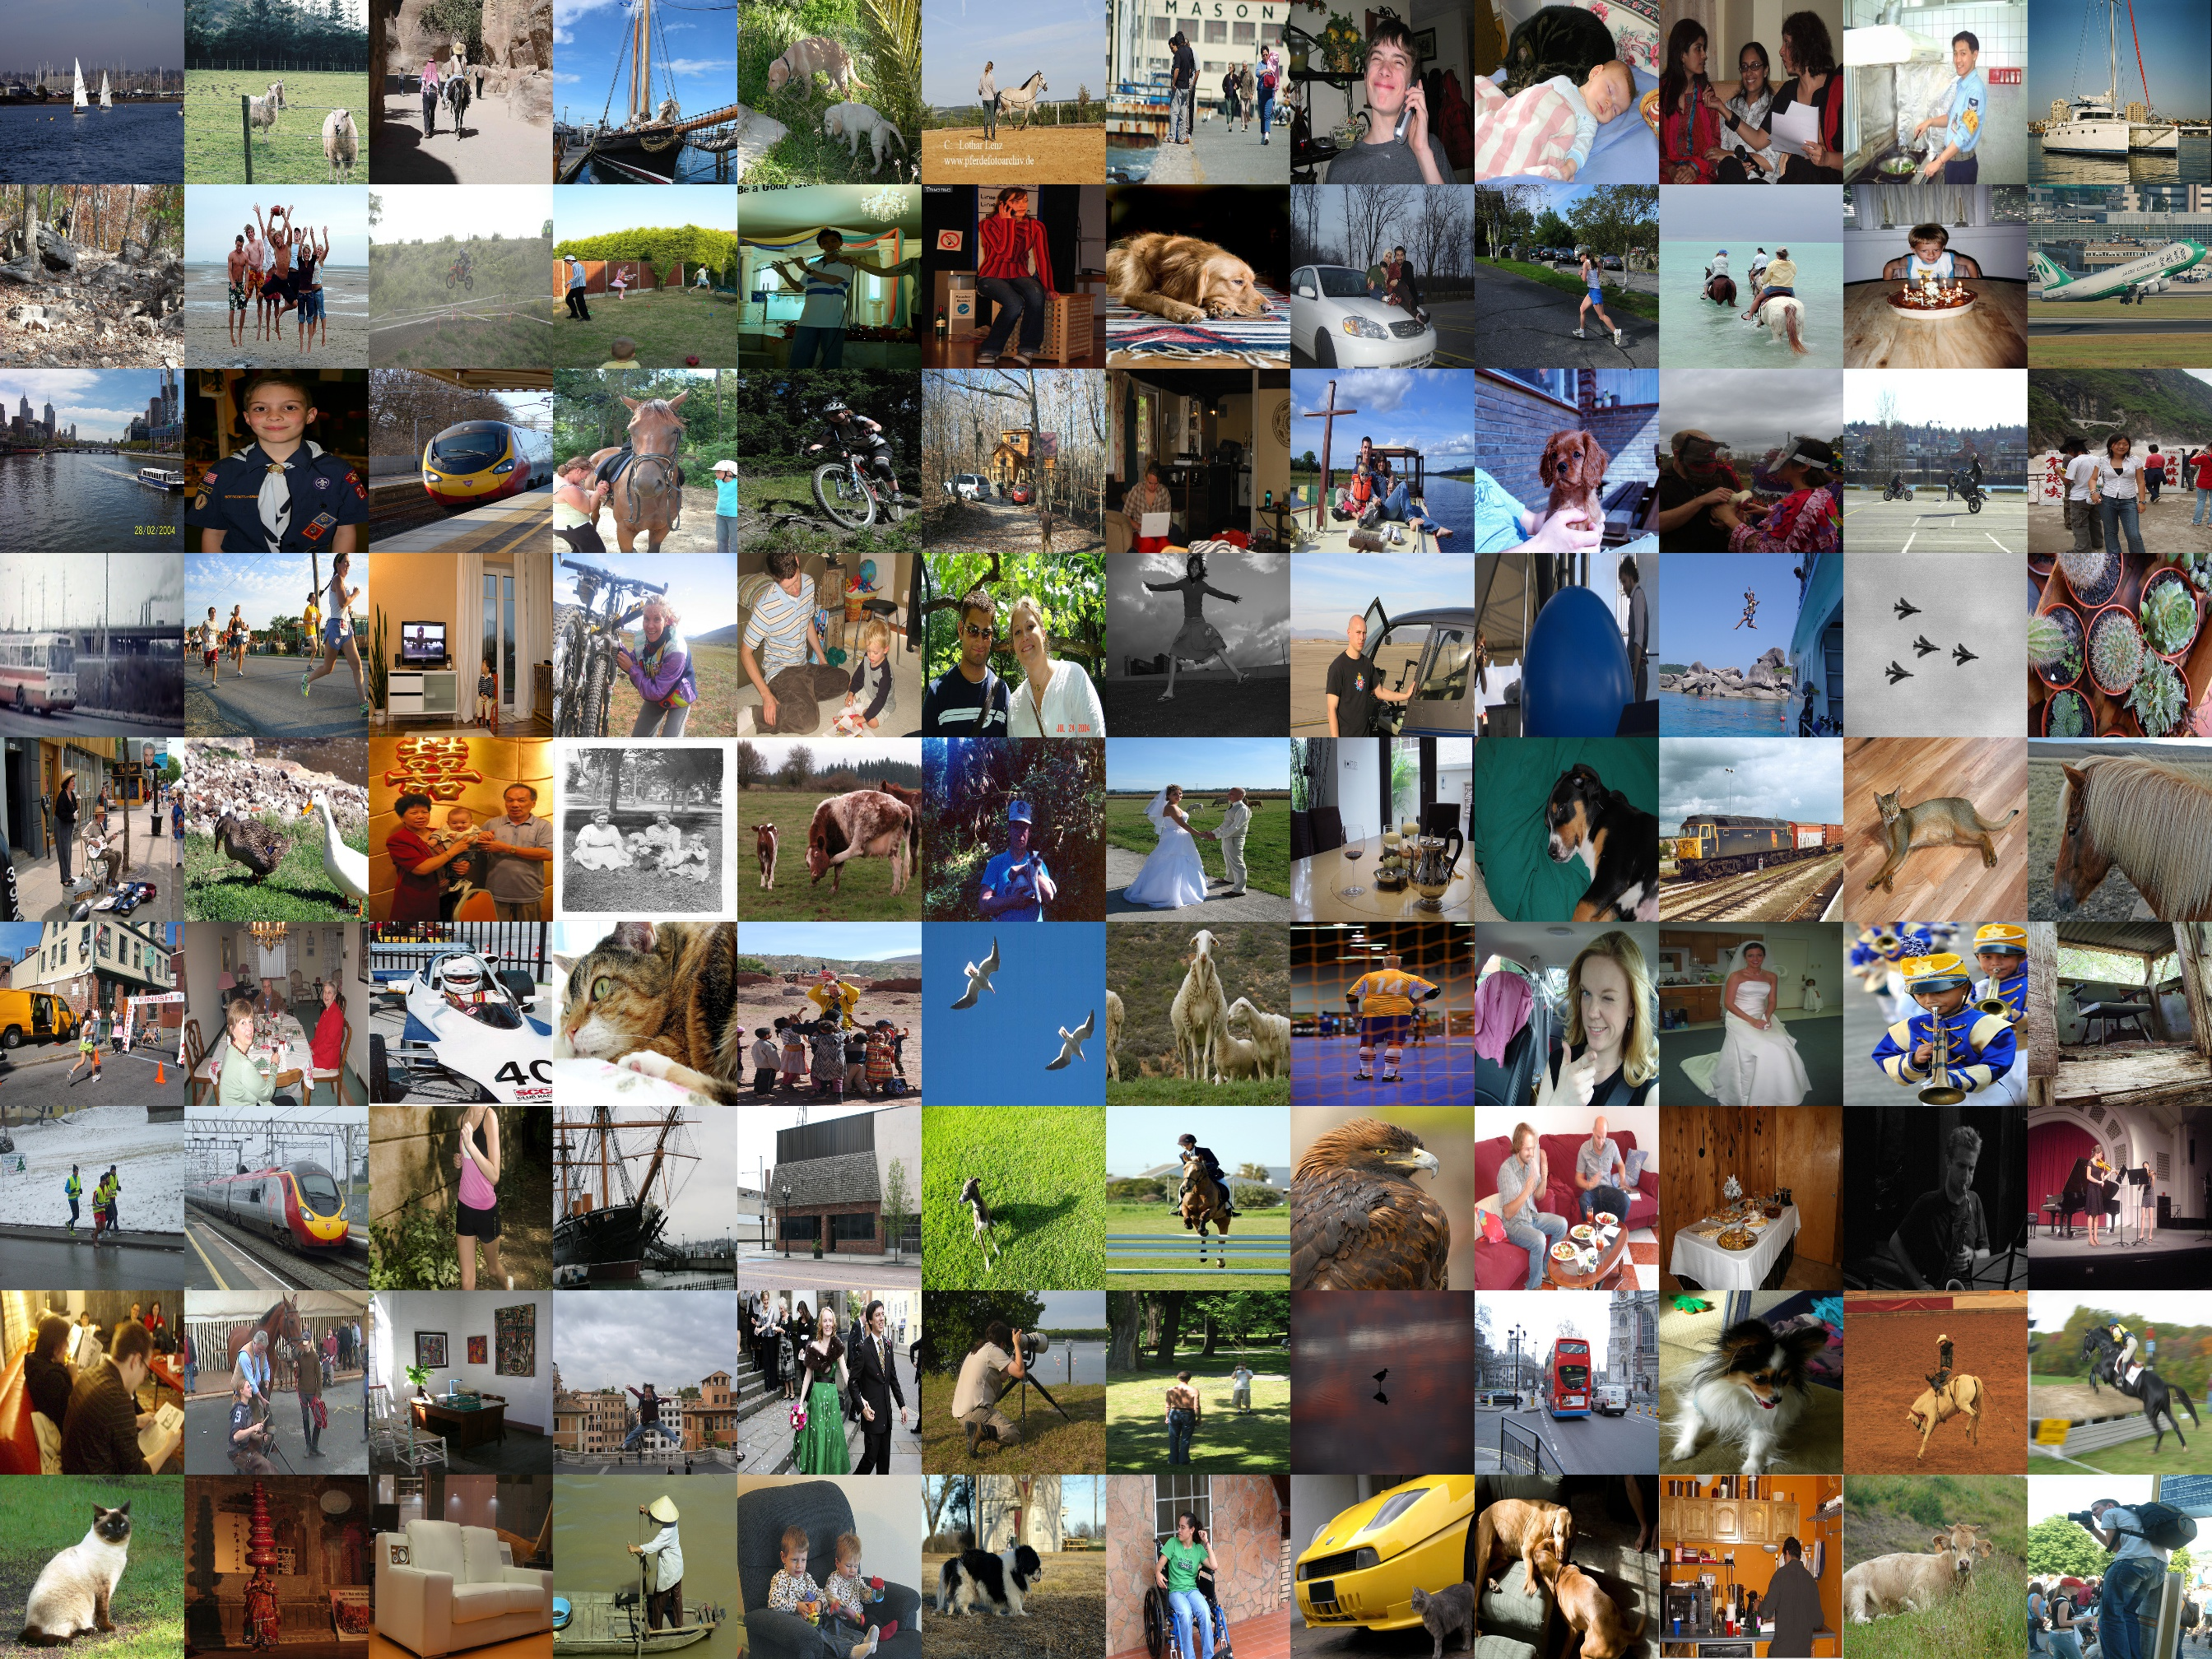
\includegraphics[width=0.5\textwidth]{sample_image}
	  \caption{\textbf{Sample synthetic image used for  performance evaluation and profiling}}
	  \label{fig:sapmle_image}
\end{figure}

*THe tables that show the effective resolution of models*
\begin{figure}[htpb]
	  \centering
	  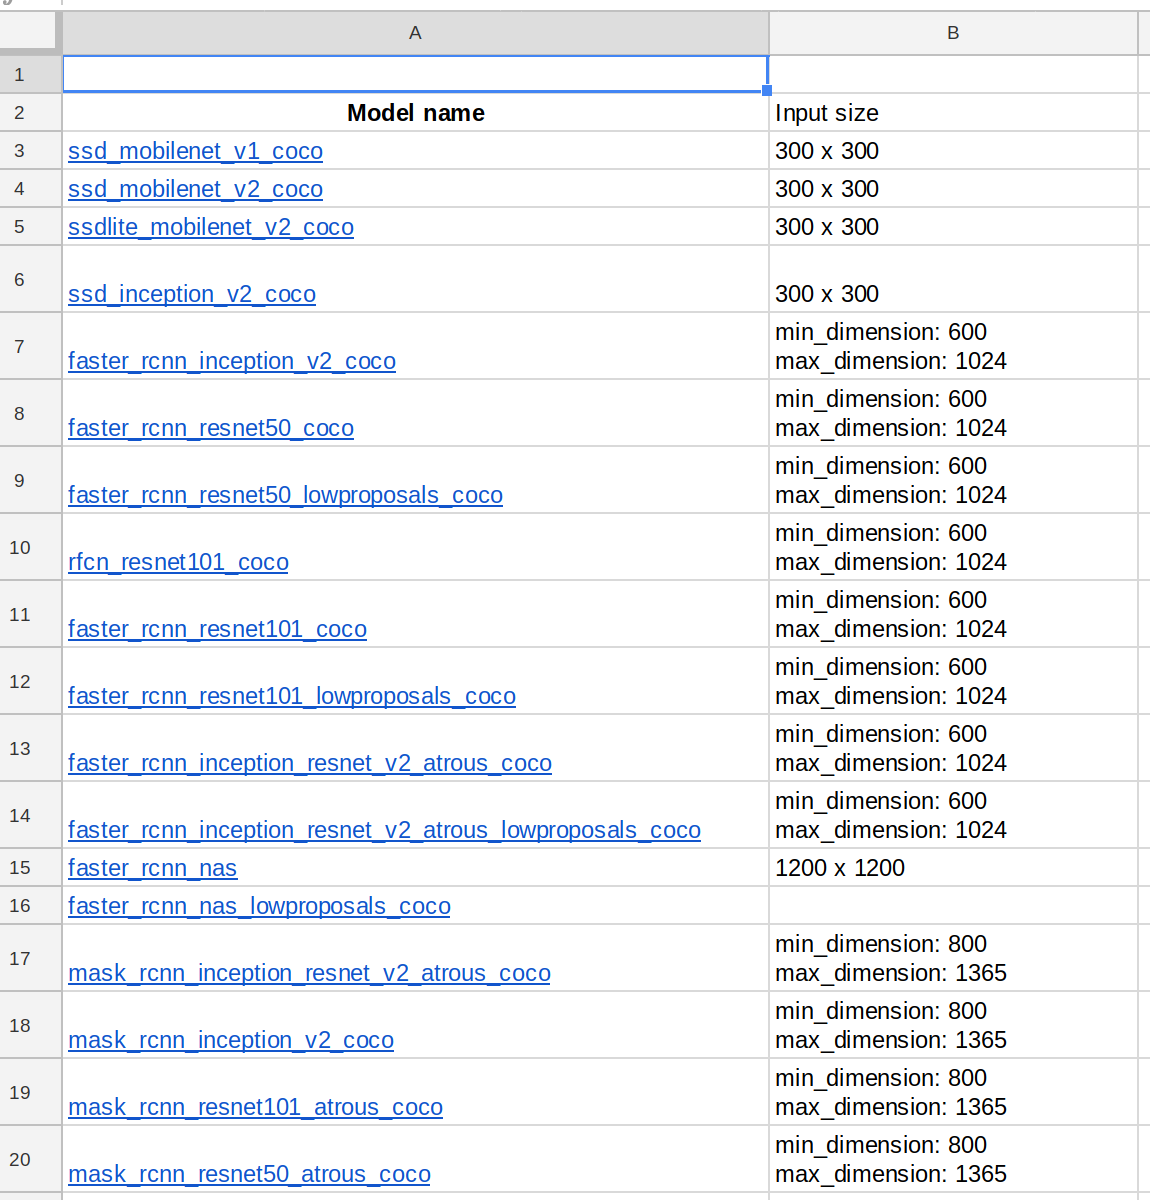
\includegraphics[width=0.5\textwidth]{model_input_size}
	  \caption{\textbf{Effective Input Sizes of different models}}
	  \label{fig:model_input_size}
\end{figure}

*Reasoning why splitting into small images is a good tactic*

%%%%%%%%%%%%%%%%%%%%%%%%%%%%%%%%%%%%%%%%%%%%%%%%%%%%%%
\section{Devices and Environment Setup}
%%%%%%%%%%%%%%%%%%%%%%%%%%%%%%%%%%%%%%%%%%%%%%%%%%%%%%

\subsection{Deep Learning Frameworks}
DeepX Toolkit is a framework used in resource efficiency deep learning optimization.

In this paper, we investigate 2 of common frameworks for deep learning applications: TensorFlow and Pytorch.

*Reasoning why we choose Tensorflow*

\subsection{Devices}
In this section, we present the comparison between detailed specification devices

\subsubsection{NVIDIA V100}

\subsubsection{NVIDIA P100}

\subsubsection{NVIDIA TX2}

%%%%%%%%%%%%%%%%%%%%%%%%%%%%%%%%%%%%%%%%%%%%%%%%%%%%%%
\section{Performance Metrics and Profiling}
%%%%%%%%%%%%%%%%%%%%%%%%%%%%%%%%%%%%%%%%%%%%%%%%%%%%%%

\subsection{Accuracy on ImageNet}
The common metric to measure accuracy in object detection is mAP, a common accuracy metric used in computer vision community.

The performance on ImageNet of several models in this paper are reported in original papers and other researches~\cite{huang2017speed}.

\dungnote{I will write this part}

\subsection{Inference Time and Memory Consumption}
In this section, we describe how we define and calculate the inference time and memory consumption of experimental models.



\subsubsection{Inference Time}

\subsubsection{Memory Consumption}
In the default configuration, Tensorflow consumes all available GPU memory resources, which mean the memory utilization would be nearly $100\%$ during all run-times.


%%%%%%%%%%%%%%%%%%%%%%%%%%%%%%%%%%%%%%%%%%%%%%%%%%%%%%
\section{Experimental Results and Analysis}
%%%%%%%%%%%%%%%%%%%%%%%%%%%%%%%%%%%%%%%%%%%%%%%%%%%%%%

% How separated parts ...

In this section, we discuss the experimental results and analyze these results in multiple perspectives and criterias.

\begin{figure}[htpb]
	  \centering
	  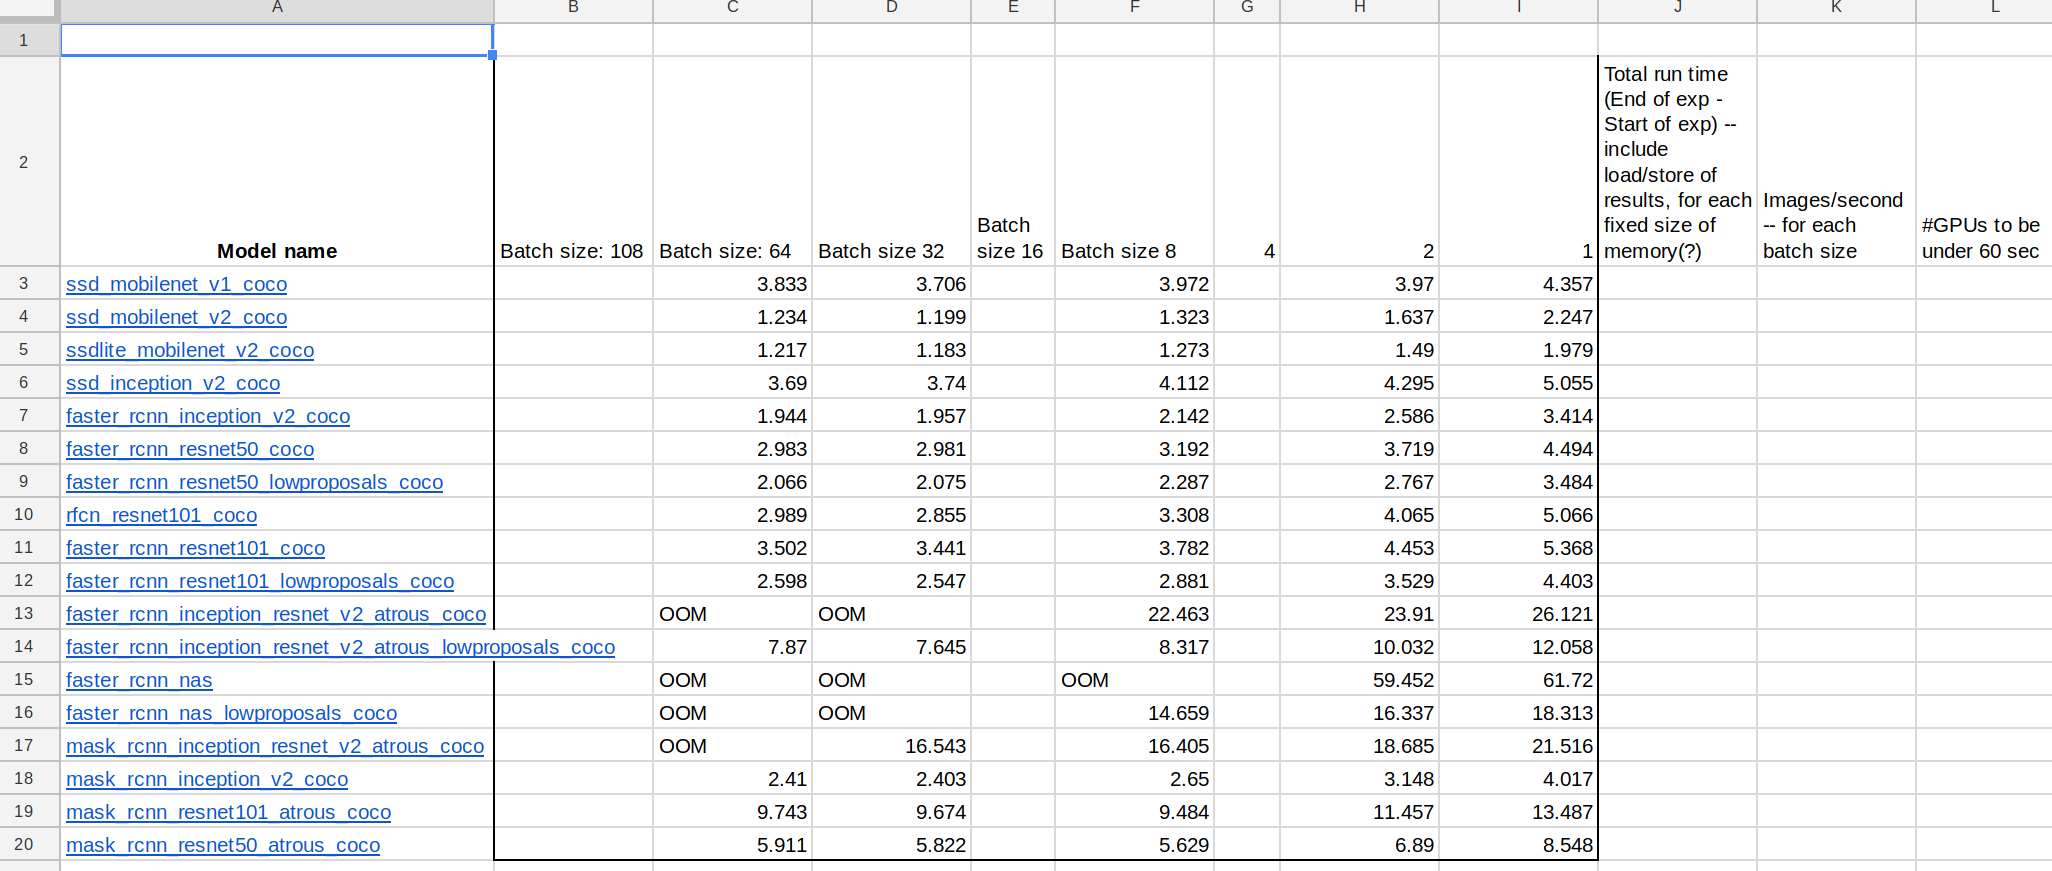
\includegraphics[width=0.5\textwidth]{experimental_results}
	  \caption{\textbf{Raw experimental results}}
	  \label{fig:experimental_results}
\end{figure}

\subsection{Inference Time and Accuracy}
This subsection draws a graph of inference time and accuracy of all models with different batch size.

\begin{figure}[htpb]
	  \centering
	  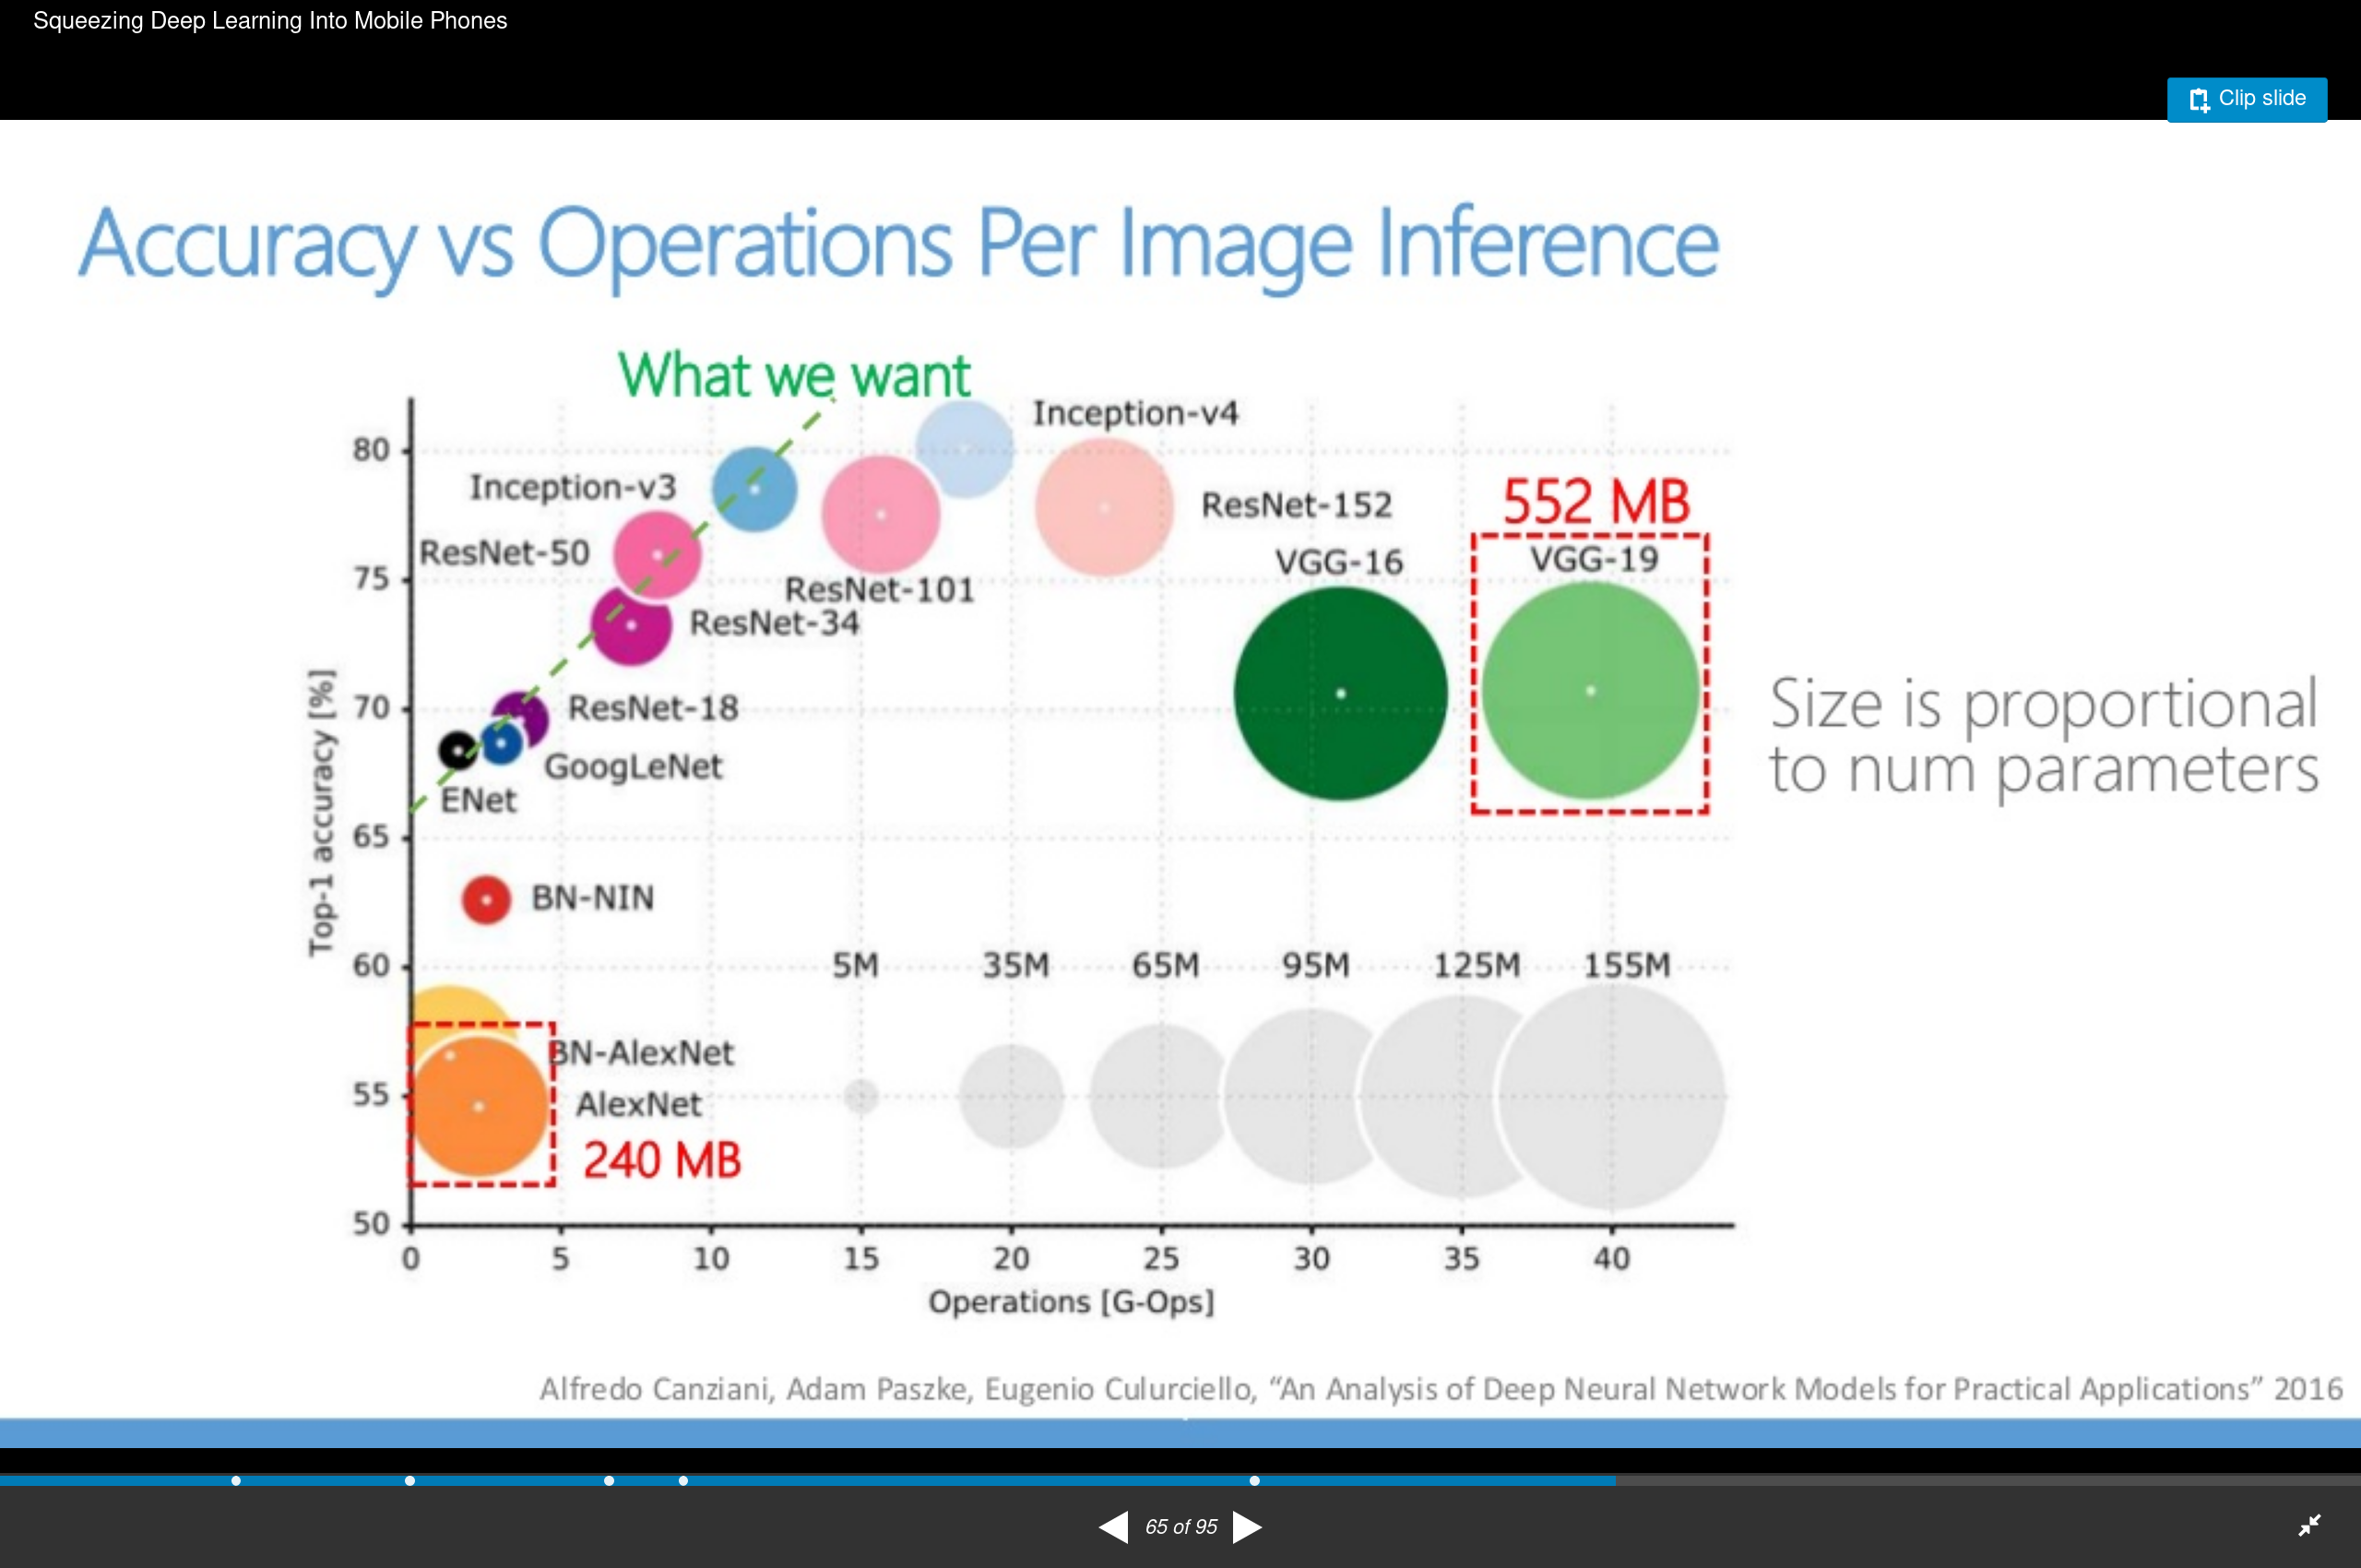
\includegraphics[width=0.5\textwidth]{time-memory-accuracy}
	  \caption{\textbf{Note: Fake diagram. Real diagram will be similar.} The correlaration between inference time and memory and accuracy}
	  \label{fig:time-memory-accuracy}
\end{figure}


\subsection{Memory Consumption and Accuracy}
This subsection draws a graph of memory consumption and accuracy of all models with different batch size.

\subsection{Inference Time and Memory Consumption}
This subsection draws a graph of memory consumption and inference time of all models with different batch size.

\subsection{Inference Time and Accuracy with restricted Memory Consumption}
This subsection draws a graph of largest batch sizes that fit into a limited amount of memory of all models with their inference time and accuracy.

\subsection{Accuracy within Time Restriction}
This subsection draws a graph of maximum accuracy that can be achieved by different time restrictions. 

%%%%%%%%%%%%%%%%%%%%%%%%%%%%%%%%%%%%%%%%%%%%%%%%%%%%%%
\section{Related Works}
%%%%%%%%%%%%%%%%%%%%%%%%%%%%%%%%%%%%%%%%%%%%%%%%%%%%%%
~\cite{huang2017speed}~do a similar research, but their experiments are limited to powerful workstations, in which the implementations of the models are developed using Tensorflow framework. The accuracy of this paper's models are evaluated on COCO for object detection.

Benchmarking deep learning system is investigated

\begin{itemize}
    \item MLPerf
    \item DeepBench
    \item Huang~\cite{DBLP:journals/corr/HuangRSZKFFWSG016} investigates the speed/accuracy trade-off f
\end{itemize}

In contrast to the approaches referenced above our benchmark is 


%%%%%%%%%%%%%%%%%%%%%%%%%%%%%%%%%%%%%%%%%%%%%%%%%%%%%%
\section{Conclusion}
%%%%%%%%%%%%%%%%%%%%%%%%%%%%%%%%%%%%%%%%%%%%%%%%%%%%%%


\bibliographystyle{unsrt}
%\bibliographystyle{abbrv}
%\setstretch{1}
%\setlength\bibitemsep{0pt}
\bibliography{deeplearning}




% that's all folks
\end{document}

